\chapter{Program and Data Modularity}
\label{c:program}

RuleWorks makes possible explicit partitioning of rules and objects
into modular systems or subsystems. The basic unit of modularity is
the \emph{block}; RuleWorks provides three block constructs:

\begin{itemize}
\item\tt{ENTRY-BLOCK}
\item\tt{DECLARATION-BLOCK}
\item\tt{RULE-BLOCK}
\end{itemize}

\begin{note}
  Blocks cannot be nested; no block may contain another block.
\end{note}

The most important type of block is the entry block. The entry block
allows a rule-based routine to be called like a routine in any other
language.

The purpose of declaration and rule blocks is to allow controlled
sharing of information.  Declaration blocks enable declarations and
the objects described by them to be shared by multiple entry or rule
blocks with the \tt{USES} clause (see Example~\ref{e:5-1}). Rule
blocks enable rules to be shared among multiple entry blocks with the
\tt{ACTIVATES} clause. Except for this sharing, the contents of one
block are not visible to other blocks.

Each block begins with a block construct that defines the block name,
and ends with an \tt{END-BLOCK} construct. A block is said to
\emph{contain} all the constructs between its block construct and its
\tt{END-BLOCK} construct. All non-block RuleWorks constructs must be
contained in a block.

\begin{tabularx}{\columnwidth}{Xlll}
  \toprule
  & Entry Block & Rule Block & Declaration Block \\
  \midrule
  Can be called from other languages & true & false & true, but* \\
  Name is visible to linker & true & true & true \\
  Can contain \verb|ON-| statements & true & false & false \\
  Can contain rules and catchers & true & true & false \\
  Can contain declarations & true & true & true \\
  Contents can be shared at compile time & false & false & true \\
  \bottomrule
\end{tabularx}

* A declaration block can be called, but only for the purpose of
initializing working memory and object classes before calling API
routines that affect working memory.

\section{Entry Blocks}

A RuleWorks \emph{entry block} generates a C-callable entry point. An
entry block is visible to your system linker and is callable by any
language that adheres to the target system's calling standard
conventions. An entry block can accept arguments and return a
value. You can think of an entry block as a rule-based subroutine or
``mini-expert.''

At least one entry block is required for each RuleWorks program.

Only one entry block can be running at any given time. The entry block
that is currently running is called the \emph{active} entry
block. Only rules contained in or activated by the active entry block
can execute. Using entry blocks to divide your program into modules
can therefore improve program performance, because the size of the
match network and the conflict set are reduced.

\subsubsection{Declaring An Entry Block}

An entry block is declared by the keyword \tt{ENTRY-BLOCK} followed by
the name of the entry block. The entry block name must contain only
letters, numbers, and underscores, and must be no longer than 31
characters.

The complete syntax of an entry block is shown in Figure~\ref{f:5-1}.

\begin{figure}[h]
  \centering
  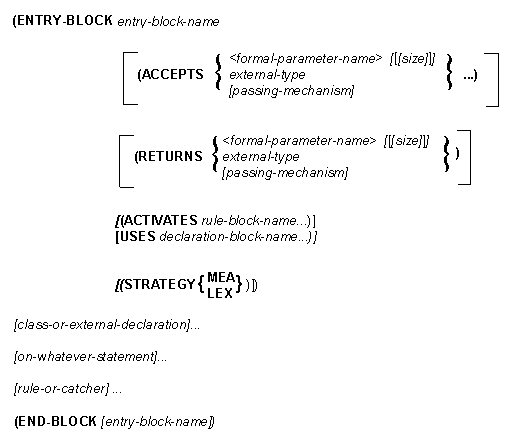
\includegraphics[scale=0.7]{f5-1}
  \caption{Entry Block Syntax}
  \label{f:5-1}
\end{figure}

The clauses within the \tt{ENTRY-BLOCK} declaration are all optional:

\begin{itemize}
\item The \tt{ACCEPTS} clause defines the input argument list, if
  any. If any argument is an array, its size is optional. See
  Chapter~\ref{c:otherlang} for information on external data types and
  passing mechanisms.
\item The \tt{RETURNS} clause specifies the entry block's return
  value, if any. If the return value is compound, its size can be
  either an input argument of an integer type (byte, short, and so on)
  or an integer constant. See Chapter~\ref{c:otherlang} for
  information on external data types and passing mechanisms.
\item The \tt{ACTIVATES} clause enables rules not contained in the
  entry block to fire. See Rule Blocks for information on rule blocks.
\item The \tt{USES} clause allows rules contained in the entry block
  to match and manipulate objects whose class declarations are not
  contained in the entry block, and to call external routines whose
  declarations are not contained in the entry block. See Declaration
  Blocks for more information on declaration blocks.
\item The \tt{STRATEGY} clause allows you to specify a
  conflict-resolution strategy other than the default \tt{MEA}
  strategy.
\end{itemize}
  
An entry block may contain any RuleWorks program constructs except
another block construct, but they must be in the order shown above:
declarations first, then \tt{ON-} statements, then rules and catchers.

If an entry block contains \tt{OBJECT-CLASS} declarations, objects of
those classes can be matched only by rules contained in the block.  If
an entry block contains rules, those rules can fire only when the
block is active.  Declaration blocks and rule blocks allow you to
share objects and rules among multiple entry blocks.

The \tt{END-BLOCK} construct is required. \it{The entry-block-name} is
optional inside the \tt{END-BLOCK} construct, but if it is present the
compiler verifies that it is the same name as in the \tt{ENTRY-BLOCK}
construct.

\subsubsection{Calling an Entry Block}

When an entry block is called, that entry block is the only active
entry block. The entry block first runs its \tt{ON-ENTRY} actions (if
any), then runs recognize-act cycles until one of the following
occurs:
\begin{itemize}
\item The conflict set becomes empty, triggering the actions that were
  declared with the \tt{ON-EMPTY} statement (if any) followed by the
  actions that were declared with the \tt{ON-EXIT} statement (if any.)
\item The \tt{RETURN} action is executed, triggering the actions that
  were declared with the \tt{ON-EXIT} statement (if any.)
\end{itemize}

Entry blocks can call other entry blocks, and even call themselves
recursively. When an entry block is called, the caller is no longer
active. The caller is referred to as being \emph{suspended} and the
called block becomes the \emph{active} block, just as with a routine
in any other language. Similarly, when the called block returns, the
caller becomes active again.

When an entry block returns, any objects created or changed by that
block remain in working memory (unless that entry block is the main
program, see Naming an Entry Block \tt{MAIN}, for details.) If
that entry block is called again later, all of those objects are again
matchable. However, the objects cannot be matched or modified by any
other entry block unless both entry blocks are using the same
declaration block (see Declaration Blocks, for information on
declaration blocks.)

\subsubsection{Scope of Arguments to an Entry Block}

The arguments received by an entry block are visible only to actions
within the \tt{ON-ENTRY}, \tt{ON-EVERY}, \tt{ON-EMPTY}, and
\tt{ON-EXIT} statements inside the entry block. They are not visible
to rules contained in or activated by the entry block. If rules need
to match input arguments, their values must be placed into one or more
objects (as shown in Example~\ref{e:5-1})

\begin{example}[!h]
\begin{quote}
\begin{verbatim}
; Shareable Class Declaration
(declaration-block numbers)
(object-class limit ^value)
(end-block numbers)

; Entry Point Declaration
(entry-block count_to
    (accepts <num-arg> long)
    (returns long)
    (uses numbers))

; Private Class Declaration
(object-class iterator ^count)

; Executable Constructs
(on-entry
    (bind <limit> (make limit ^value <num-arg>))
    (make iterator ^count 1))

(on-exit
    (remove <limit>) ; clean out WM when done
    (return <num-arg>))

(rule increment-rule
    (limit ^value <lim>)
    (iterator ^$id <it> ^count { <num> <= <lim> })
  -->
    (modify <it> ^count (<num> + 1)))

(rule now-done
    (limit ^$id <limit-id> ^value <lim>)
    (iterator ^$id <it> ^count > <lim>)
  -->
    (remove <it>)
    (remove <limit-id>))

(end-block count_to)
\end{verbatim}
\end{quote}
\caption{A Simple Entry Block and Declaration Block}
\label{e:5-1}
\end{example}

The same restrictions hold true of any variables bound in an \tt{ON-}
clause. Such variables are also visible within any \tt{ON-} clause.

\subsubsection{Scope of Execution of Entry Blocks}

A \emph{call frame} is created when a RuleWorks entry block is
called. It contains all the dynamic data structures associated with a
given invocation of an entry block. That is, it consists of all of the
information ``local'' to this particular invocation of an entry block,
or in some way visible to this particular invocation. Calls and
returns really create and delete call frames. Call frames are an
integral piece of entry blocks; by themselves they have no names and
cannot be passed, returned, or otherwise manipulated directly.

The following are local to the call frame:
\begin{itemize}
\item Refraction.

  Refraction does not apply across invocations of entry blocks. Thus,
  a rule may fire more than once on the same data.  This could happen
  when an entry block calls itself recursively, or when one entry
  block calls another and both activate the same rule block, or when
  an entry block is called repeatedly.

\item The local rule-firing counter.

  This affects \tt{CATCH} statements. The \tt{CATCH} counter counts
  only rules fired in the entry block invocation in which the
  \tt{AFTER} action was executed, excluding rule firings in other
  invocations of the same entry block and in entry blocks called from
  the original entry block.
\end{itemize}

The following are global:
\begin{itemize}
\item The \verb|$ID| generator.

  The \verb|$ID| value of an object is universally unique across entry
  block invocations.

\item The time-tag counter.

  The time-tags assigned to objects are monotonically increasing
  across calls to and returns from entry blocks.

\item The global rule-firing counter.

  This affects the \tt{RUN} command when you provide an argument (for
  example, \tt{RUN} 5).  Rule firings from other entry blocks are
  counted.

\item The atom generator.

  This affects the RuleWorks \tt{GENATOM} and \tt{GENINT} functions,
  and the \verb|rul_genint|, \verb|rul_gensym|, and \verb|rul_gensymp|
  API routines.  Every atom generated for any of these routines is
  unique while the program is running, and is unique across your
  entire program, not merely within an entry block.
\end{itemize}

\subsubsection{Naming an Entry Block \tt{MAIN}}

An entry block named \tt{MAIN}, if supplied, is automatically
designated to the compiler and linker as the main RuleWorks
routine. This design has semantic parallelism with the C language and
provides the behavior most programmers would expect. The name can be
in any case.

If you want to capture command-line arguments to the program in a
portable way, a declaration in the following form is recommended:
\begin{quote}
\begin{verbatim}
(entry-block main
    (accepts <argc> long            ; traditional names for
             <argv> [<argc>] ASCIZ) ; command-line args
     ...)
\end{verbatim}
\end{quote}

\subsubsection{Returning a Value from an Entry Block}

RuleWorks provides an RHS action, \tt{RETURN} that stops the firing of
rules in the active entry block, executes the \tt{ON-EXIT} actions (if
any) and passes control back to the caller of the entry block. This
action has an optional argument, the value to be returned. The
argument can be any expression. Thus, the \tt{RETURN} action is useful
for returning a condition code or value (see Example~\ref{e:5-1}).

The \tt{RETURN} action is valid anywhere in the entry block, even
inside the \tt{ON-EXIT} and \tt{ON-EMPTY} statements. The \tt{RETURN}
action is valid only in an entry block; it is not valid in a rule
block.

Executing more than one \tt{RETURN} action in an entry block is
possible, for example, when an \tt{ON-EXIT} statement that contains a
\tt{RETURN} action is executed as a result of a \tt{RETURN} action in
a rule. If a value is being returned from the entry block, the value
of the last \tt{RETURN} action executed is used.

If the value returned by an entry block is an array, the memory
allocated for that array is not freed by RuleWorks. The following
example shows an entry block that accepts an array, sorts it, and then
returns it.

\begin{quote}
\begin{verbatim}
(entry-block sort_slowly
    (accepts <set-size> long
             <set>[<set-size>] asciz)
    (returns <sorted-set>[<set-size>] asciz))

; Return the input set, except sorted (albeit slowly)
(object-class an-atom ^value)

(object-class in-set ^values compound)

(object-class out-set ^values compound)

(on-entry
    (make out-set)
    (make in-set ^values <set>)
    (for-each <atom> in <set>
        (make an-atom ^value <atom>)))

(rule find-next
    (an-atom ^$id <atom> ^value <x>)
    -(an-atom ^$id <> <atom> ^value <= <x>)
    (out-set ^$id <out-set> ^values <out-vals>)
  -->
    (remove <atom>)
    (modify <out-set> ^values (compound <out-vals> <x>)))

(rule all-done
    (out-set ^$id <out-set> ^values <out-vals>)
    (in-set ^$id <in-set> ^values <in-vals>)
    -(an-atom)
  -->
    (remove <out-set> <in-set>)
    (write (crlf) | Sort of | <in-vals>
      (crlf) | ==> | <out-vals> (crlf))
    (return <out-vals>))

(end-block)
\end{verbatim}
\end{quote}

\section{Executing Actions Without Matching}

The actions on the right-hand side of a rule are executed only when
the left-hand side matches working memory and the resulting
instantiation is picked during conflict resolution. RuleWorks provides
two types of executable constructs whose actions are executed without
matching working memory: \tt{ON-} statements and catchers.

\subsubsection{Using \tt{ON-} Statements}

RuleWorks entry blocks may contain one each of the four \tt{ON-}
statements, which allow you to describe a set of actions that are
executed at certain points in the recognize-act cycle (see the figure,
\tt{ON-} Statements and the Recognize-Act Cycle) without matching
any objects in working memory. These new statements are all defined
with names that begin with the prefix \tt{ON-} and end with the name
of the special condition under which their associated actions are
executed.

\begin{figure}
  \centering
  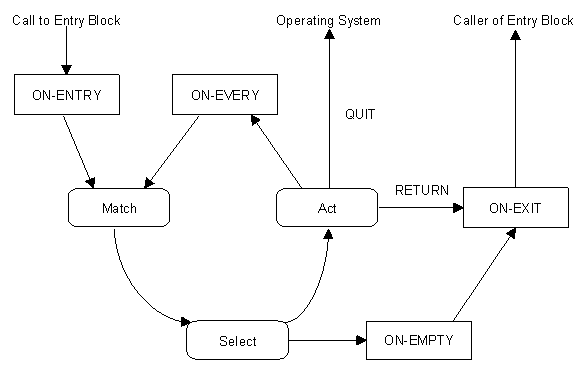
\includegraphics[scale=0.7]{f5-2}
  \caption{\tt{ON-} Statements and the Recognize-Act Cycle}
  \label{f:5-2}
\end{figure}

The "\tt{ON-}" statements are listed below:
\begin{itemize}
  \item \tt{ON-ENTRY}

    The actions in an \tt{ON-ENTRY} statement are executed whenever
    its entry block is called, and before any rules can fire.  Thus,
    you can initialize working memory by putting \tt{MAKE} actions in
    your \tt{ON-ENTRY} statement. For example:

    \begin{quote}
\begin{verbatim}
(on-entry
    (bind <my_id> (make my_wmo)) ; Create the first WMO.
    (bind <rule_count> 0)        ; Initialize the counter...
    (bind <return_status> good)) ; ... and the return value.
\end{verbatim}
    \end{quote}

These \tt{MAKE} actions can use the input arguments to the entry block
(see the section of this chapter, Scope of Arguments to an Entry
Block)

The \tt{ON-ENTRY} statement is roughly analogous to the OPS5
\tt{STARTUP} statement.

\item \tt{ON-EVERY}

  The actions in an \tt{ON-EVERY} statement are executed immediately
  after each successful rule firing, and before the determination of
  the next rule to fire. If a rule is fired that has a \tt{RETURN} as
  its last action, then control will be returned up to the caller, and
  the \tt{ON-EVERY} actions will not be executed.

  You could use an \tt{ON-EVERY} statement to count the number of
  rules fired in the current invocation of the entry block, or to call
  an event handler. For example:
  \begin{quote}
\begin{verbatim}
(on-every
    (bind <rule-count> (<rule-count> + 1)))
\end{verbatim}
  \end{quote}
        
\item \tt{ON-EMPTY}

  The actions in an \tt{ON-EMPTY} statement are executed whenever it
  is time to select the next rule to fire and there are no rules
  eligible to fire and thus the conflict set is empty. Note that the
  run-time system does not execute any recognize-act cycles after an
  \tt{ON-EMPTY} statement, even if its actions create WMOs that
  satisfy one or more rules.

  You could use an \tt{ON-EMPTY} statement to return a failed status
  if the program should not have arrived at an empty CS.  For example:
  \begin{quote}
\begin{verbatim}
(on-empty
    (quit $failure))
\end{verbatim}
  \end{quote}
        
\item \tt{ON-EXIT}

  The actions in an \tt{ON-EXIT} statement are executed just before
  control is returned to the caller of the entry block. These actions
  are executed when control is returned via a \tt{RETURN} action or
  when the conflict set becomes empty. If an \tt{ON-EMPTY} statement
  was also specified, the \tt{ON-EXIT} actions are executed after the
  \tt{ON-EMPTY} actions, and immediately before control is returned to
  the calling routine.

  The \tt{ON-EXIT} actions are not executed after a \tt{QUIT} action
  or command.

  \tt{ON-EXIT} statements are useful for clean-up actions, such as
  removing dead instances of local object classes. For example:

  \begin{quote}
\begin{verbatim}
(on-exit
    (remove <my_id>)
    (remove-every local)
    (return <return_status>))
\end{verbatim}
  \end{quote}

\end{itemize}

\tt{ON-} statements must be contained in an entry block. They cannot
appear inside a rule block, nor inside a rule group within an entry
block (see Rule Blocks and Rule Groups for more information.)

\begin{note}
  Any variables bound in one \tt{ON-} statement are available to all
  other \tt{ON-} statements. These variables are not available to any
  rules.
\end{note}

An entry block can contain at most one of each type of \tt{ON-}
statement. It doesn't have to contain any of them.

\subsubsection*{Using a Catcher}

A \emph{catcher} is a list of actions that are executed after a
specified number of recognize-act cycles have been executed. For
example, if program execution is unattended, as in a batch job, a
catcher can halt the program if it does not produce results within a
specified limit.

You define a catcher with a \tt{CATCH} statement, which includes a
symbol and one or more actions. The symbol names the catcher, and
functions as a label. A catcher's name must be unique; that is, it
cannot be the same as the name of another catcher, rule, or rule group
in the program. When the catcher fires, the actions are executed.

The following \tt{CATCH} statement defines a catcher named
\tt{FINISH}, which consists of two actions, \tt{WRITE} and \tt{HALT}:

\begin{quote}
\begin{verbatim}
(catch finish
    (write (crlf) |Finished.|)
    (halt))
\end{verbatim}
\end{quote}

You enable a catcher with the \tt{AFTER} action, which tells the
run-time system when to execute the catcher. Specify the \tt{AFTER}
action with a positive integer and the name of the catcher you want to
enable. The integer indicates the number of recognize-act cycles (of
the current invocation of the entry block) that the run-time system is
to execute before executing the specified catcher. For example:

\begin{quote}
\begin{verbatim}
(after 10 finish)
\end{verbatim}
\end{quote}

Only one catcher can be enabled at a time, per call frame. Therefore,
when you enable a catcher, you disable the catcher currently enabled
(if any.) Catchers are automatically disabled after they have been
executed.

Catchers may be contained in either entry or rule blocks. The catcher
must be contained in the same block as the \tt{AFTER} action that
enables it.

The following example illustrates the use of two catchers,
\tt{STARTER} and \tt{FINISH}.

\begin{quote}
\begin{verbatim}
(entry-block sample)

(object-class start) ; Used for initialization

(object-class number ^value) ; Contains value to be printed

(on-entry
    ; Creates a working-memory object (START)
    (make start)
    ; Enables catcher STARTER after 1 recognize-act cycle
    (after 1 starter))

(2) (catch starter ; Catcher STARTER
        (write (crlf) |Counting to 10...|)
        (make number ^value 1)
        ; Enables catcher FINISH after the run-time
        (after 10 finish))

    ;system has executed 10 more cycles
(4) (catch finish ; Catcher FINISH
        (write (CRLF) |Finished.|)
        (return)) ; Stop program

(1) (rule initialize ; Initialize working memory
        (start ^$id <START>)
      -->
        (write (crlf) |Starting...|)
        (remove <start>))

(3) (rule count ; Output numbers
        (number ^$id <number> ^value <n>)
      -->
        (write (crlf) (rjust 5) <n>)
        (modify <number> ^value (<n> + 1)))

(end-block sample)
\end{verbatim}
\end{quote}

This program produces the following output:

\begin{quote}
\begin{verbatim}
Starting...
Counting to 10...
     1
     2
     3
     4
     5
     6
     7
     8
     9
     10
Finished.
\end{verbatim}
\end{quote}

\tt{STARTER} and \tt{FINISH} are used as follows:
\begin{itemize}
\item[\tt{(1)}] The first recognize-act cycle fires rule
  \tt{INITIALIZE}, because its CE matches the \tt{START} object
  created in the \tt{ON-ENTRY} statement. The \tt{ON-ENTRY} statement
  does not count as a cycle.

\item[\tt{(2)}] Catcher \tt{STARTER} fires after one recognize-act
  cycle has been executed. \tt{STARTER} is enabled in the
  \tt{ON-ENTRY} statement.

\item[\tt{(3)}] The \tt{MAKE} action in catcher \tt{STARTER} creates
  an object on which rule \tt{COUNT} can fire.

\item[\tt{(4)}] The \tt{AFTER} action in catcher \tt{STARTER} enables
  catcher \tt{FINISH} to fire after ten more recognize-act cycles have
  been executed.
\end{itemize}

\section{Declaration Blocks}

Declarations (\tt{OBJECT-CLASS} and \tt{EXTERNAL-ROUTINE}) can be
private or shareable.  A declaration is \emph{private} if it is
contained in either an entry block or a rule block. Objects whose
class declaration is private to a block can be matched only by rules
contained in that block. In other words, by placing declarations
inside an entry block or rule block you create private data for that
block. Similarly, external routines whose declarations are local to a
block can be called from inside that block only.

Figure~\ref{f:5-3} shows a RuleWorks program that consists of one
entry block with two private object class declarations. Rules in
\tt{EB1} can ``see'' all objects of classes \tt{Y} and \tt{Z}.

\begin{figure}[h]
  \centering
  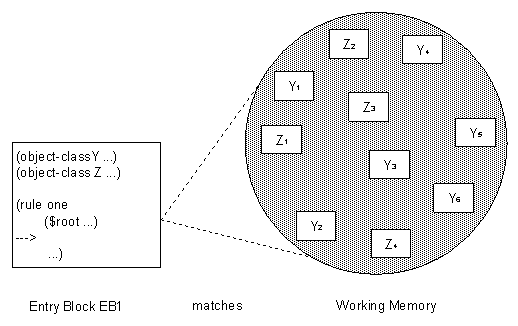
\includegraphics[scale=0.7]{f5-3}
  \caption{Private Data in RuleWorks}
  \label{f:5-3}
\end{figure}

\subsubsection{Data Partitioning}

By default, RuleWorks partitions working memory so there is no
conflict over object classes of the same name when two or more entry
blocks are combined. Rules can match only objects whose classes are
contained in or used by their entry block; all other objects are
invisible.

This invisibility includes matches against the built-in class
\verb|$ROOT|. If an object class is not visible at compile-time,
instances of it are not visible to the block at run-time.

\subsubsection{Declaration Sharing}

A \emph{declaration block} allows you to create a collection of
declarations that are \emph{shareable} among multiple entry blocks or
rule blocks.  \emph{Declaration sharing} allows you to explicitly
decide which data should remain private and which should be shared
(and the extent of that sharing). This allows the absolute
partitioning of object class declarations between several
independently-developed subsystems of an application. It also allows
information to be restricted to a single routine or a set of
interdependent routines.

A declaration block consists of zero or more declarations bounded by a
\tt{DECLARATION-BLOCK} construct at the top and an \tt{END-BLOCK}
construct at the bottom.

\begin{quote}
\begin{verbatim}
(declaration-block line-items)

    (object-class item ^item-code
        ^item-name
        ^quantity
        ^price-per
        ^item-total)

    (object-class shippable-item
        (inherits-from item)
        ^part-number)

 (end-block line-items)
\end{verbatim}
\end{quote}

The complete syntax of a declaration block is shown below:
\begin{quote}
\verb|(|\tt{declaration-block} \it{decl-block-name}\verb|)|\par
\qquad[\it{class-or-external-declaration}] \ldots\par
\verb|(|\tt{end-block} [\it{decl-block-name}]\verb|)|
\end{quote}
 
The \it{decl-block-name} is required in the \tt{DECLARATION-BLOCK}
construct. It is optional in the \tt{END-BLOCK} construct, but if
supplied it is checked. Declaration block names must be no longer than
31 characters, and contain letters, digits, and underscores only.
Declaration block names must be distinct from entry and rule block
names. Finally, the first eight characters of all declaration block
names used in a program must be unique. This allows RuleWorks to
create portable names for the compiled files. For example, having two
declaration blocks named \verb|DECLARE_CONTROL| and
\verb|DECLARE_KIWI| generates a compile-time warning and results in a
single file called \verb|DECLARE_.USE|. Naming the blocks
\verb|CONTROL_DECLS| and \verb|KIWI_DECLS| correctly generates two
\verb|.USE| files.

\begin{note}
  Object classes that are related by inheritance must all be declared
  in the same block. An object class cannot inherit from a class
  declared in some other block.
\end{note}

A declaration block must not contain any executable statements (rules,
\tt{ON-} statements, or catchers).

Declarations are shared via the \tt{USES} clause of an
\tt{ENTRY-BLOCK} or \tt{RULE-BLOCK} construct.  Objects whose class
declarations are shared by a block are just as visible to the rules
within that block as objects whose declarations are private to that
block. Note that a \tt{USES} clause cannot specify individual class
names, only declaration block names.

A block can use more than one declaration block. A compile-time error
occurs if the combined shared and private declarations contain any
classes with identical names.

Figure~\ref{f:5-4} shows some private and some used object class
declarations. The \tt{USES} clause in \tt{EB1} ``pulls in'' the
declarations from \tt{DB1}.  Rules in \tt{EB1} can still match objects
of classes \tt{Y} and \tt{Z}.

\begin{figure}[h]
  \centering
  \input f5-4.tex
  \caption{Shareable Declaration Blocks}
  \label{f:5-4}
\end{figure}

Figure~\ref{f:5-5} shows two entry blocks in the same program, each
with some private and some used object class declarations. Rules in
\tt{EB1} can see objects of classes \tt{Y} and \tt{Z} only; rules in
\tt{EB2} can see objects of classes \tt{W} and \tt{X} only.

\begin{figure}[h]
  \centering
  
\includegraphics[scale=0.5]{f5-5}
  \caption{Two Shareable Declaration Blocks}
  \label{f:5-5}
\end{figure}

Figure~\ref{f:5-6} shows the same two entry blocks sharing an object
class declaration. Rules in \tt{EB1} can see objects of classes
\tt{Y}, \tt{Z}, and \tt{O}; rules in \tt{EB2} can see objects of
classes \tt{W}, \tt{X}, and \tt{O}.

\begin{figure}[h]
  \centering
  
\includegraphics[scale=0.5]{f5-6}
  \caption{Shared Data in RuleWorks}
  \label{f:5-6}
\end{figure}

The declaration block(s) used by an entry block must be compiled
before the entry block itself can be compiled. You can put declaration
blocks in a different file and compile them separately, or you can
place them in the same file but above the entry block. In either case,
compiling a declaration block results in an intermediate file with the
extension \tt{.USE}. Entry or rule blocks in other source files can
subsequently use one or more of those declaration blocks, without
seeing all of the other declarations that were in the original source
file.

The following example shows a more complex set of block constructs where both
declarations and rules are being shared.

\begin{quote}
\begin{verbatim}
(declaration-block common_decls)
    (object-class C-1 ...)
    (object-class C-2 ...)
(end-block common_decls)

(entry-block my_little_function
    (accepts ...)
    (activates shared-rules-1)
    (uses common_decls))
    ; needed to expose the contents of the
    ; declaration-block defined above

(rule my-rule-1 ...)
...

(end-block my_little_function)

(rule-block shared_rules_1
    (uses common_decls))

(rule my-rule-1 ...)
...

(end-block shared_rules_1)

(rule-block shared_rules_2
    (uses common_decls))
...

(end-block shared-rules-2)

(entry-block my_other_little_function
    (accepts ...)
    (activates shared-rules-1 shared-rules-2)
    (uses common_decls))

(rule my-rule-1 ...)
...

(end-block my_other_little_function)
\end{verbatim}
\end{quote}

\subsubsection*{Calling a Declaration Block}

Declaration blocks are callable, and in certain circumstances it may
be necessary to call one. For example, the following C program calls
an entry block named \verb|KBT_RULES| that uses a declaration block
named \verb|KBT_DECL|. In order for the C program to initialize
working memory before calling the entry block, it must first call the
declaration block:

\begin{quote}
\begin{verbatim}
#include <stdio.h>
#include <rul_rtl.h>

main ()
{
    /* define RuleWorks stuff */
    rul_atom obj_id;

    printf("Calling RuleWorks...");

    /* initialize working memory */
    KBT_DECL();

    /* make one object */
    rul_make_instance("(AnyWin ^name testing)","KBT_DECL");
    /* call RuleWorks entry block */
    kbt_rules();
}
\end{verbatim}
\end{quote}

\section{Rule Blocks}

In RuleWorks, rules can be gathered together into \emph{rule
  blocks}. A rule block is a collection of rules that may be shared
among several entry blocks. Whenever \emph{any} of the entry blocks is
called, all the rules in the rule blocks it activates will participate
in matching and be enabled to fire.

Rule blocks can also be used when the number of rules in a single
entry block becomes too large to reasonably store in a single file.
You can have rule blocks that are activated by only one entry block.

The complete syntax of a rule block is shown in Figure~\ref{f:5-7}.

\begin{figure}[h]
  \centering
  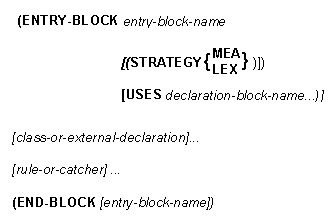
\includegraphics[scale=0.7]{f5-7}
  \caption{Complete Syntax of Rule Block}
  \label{f:5-7}
\end{figure}

Rule blocks are activated by entry blocks with the \tt{ACTIVATES}
clause. Only rules contained in or activated by the active entry block
are eligible for matching and firing. Only entry blocks can activate
rule blocks; one rule block can neither contain nor activate another.

The \it{rule-block-name} is required in the \tt{RULE-BLOCK}
construct. It is optional in the \tt{END-BLOCK} construct, but if
supplied it is checked. Rule block names must be no longer than 31
characters, and contain letters, digits and underscores only. Rule
block names must be distinct from entry and declaration block names.

Each rule block can have it's own \tt{STRATEGY} clause. However, all
rule blocks used by an entry block must have the same strategy as the
entry block. It is a run-time error to activate rule blocks that have
different strategies. If no strategy clause is specified, the default
is \tt{MEA}.

A rule cannot be in more than one rule block; a rule block can contain
zero or more rules.  (An empty rule block can be useful during
prototyping and/or stuibbing phase of development.) Note that all
rules contained in a block must be in the same file, but a file can
contain more than one block. Rule blocks can be compiled before or
after the entry block that activates them.

\begin{note}
  A rule block is not a directly callable entity, and should not be
  called from any language except RuleWorks. If a rule block is not
  referenced by at least one entry block, it's rules can never
  fire. No rules can be shared among multiple entry blocks unless they
  are contained within a rule block.
\end{note}

Rule blocks are activated by entry blocks by the \tt{ACTIVATES} clause
(see Entry Blocks). Only rules contained in or activated by the active
entry block are eligible for matching and firing. Only entry blocks
can activate rule blocks; one rule block can neither contain nor
activate another.

The visibility of objects to the active rules depends on whether their
blocks contain or use the corresponding \tt{OBJECT-CLASS}
declarations.  When you put rules in rule blocks, it is up to you to
set up declaration blocks in such a way that the classes that are to
be matched and modified in your entry and rule blocks are shared as
appropriate. There is no implicit sharing of declarations between an
entry block and the rule blocks it activates. Thus, in the example,
Sharing Declarations and Rules, the clause is required in the rule
block as well as in the entry blocks.

\section{Scope of Names}

In RuleWorks, the name space for declarations and executable
statements is not global. This name space is divided by blocks into
independent name spaces.

\begin{itemize}
\item Within a block, all named constructs except external routines
  share the same name space. Therefore, no rule can have the same name
  as another rule, rule-group, or catcher in that same
  block. Different blocks can, however, each contain a rule with the
  same name.

  This name space is enforced by the RuleWorks compiler, and permits
  names to be any legal symbol.

  When an entry block activates rule blocks, the entry block and all
  the rule blocks still have separate name spaces.

\item Object classes inhabit a second name space, which is also
  enforced by the RuleWorks compiler. You can have an object class and
  a rule with the same name, but you cannot have an object class and
  an external routine with the same name.

  When an entry block or a rule block uses declaration blocks, the
  using block and all the used blocks have one common name space for
  object classes and external routines.

\item Block names and external routine names share a third name space,
  which is enforced by the platform linker. For example, a rule block
  cannot have the same name as an entry block, declaration block, or
  external routine called by the same program.
\end{itemize}
  
\section{Rule Groups}

Within an entry or rule block, an additional level of structure can be
imposed on a collection of rules by using the \tt{RULE-GROUP}
construct. This extra level is not necessary for program execution,
but it can enable some useful debugging information.

\section{Efficiency Issues}

The entry block system in RuleWorks may cause a program speed
\emph{increase} because it restricts the visibility of rules and
objects to what you specified, rather than the global visibility of
OPS5.

Only those programs that actually use the block system will see the
efficiency improvement. Programs that are converted from OPS5 by
wrapping a single entry block around all of the rules will not see
this improvement.

The entry block system may impose an efficiency penalty when entry
blocks are called repeatedly. To avoid this problem, you should
compile any entry block that is called repeatedly with the Optimize
qualifier set to \tt{REINVOCATION}. Note that the RuleWorks language
semantics are not affected by this qualifier, only entry block
initialization run-time and maximum memory usage.

Partitioning working memory with declaration blocks will, if done
appropriately, provide a significant improvement in execution speed.

%%% Local Variables:
%%% mode: latex
%%% TeX-master: "rwug"
%%% End:
